\section{Results from Simulation}
%Previously we defined good paths in terms of the actual cost of the path in relation to the costmap. However, these metrics are not necessarily the ones we ultimately want to use when we move up to an interaction mindset. 

%\subsubsection{Path Length}
%\subsubsection{Closest Approach Distance}
%\subsubsection{Average Distance to Obstacle}

%If we were simply to accept the path with the lowest total cost as ``the best,'' we could now rest, assured that Dijkstra's algorithm would find the optimal path. However, in robotics, and particularly human robot interaction, there are other metrics that weigh on the value of a path. The one that is of most use to us here is the closest distance between the path and the obstacle. With the bracket shape we discussed earlier, that metric has the value of $\yhat$. There are many other metrics that we could consider, including the path length and the average distance from path to obstacle, however, those measures work proportionally to the closest distance in all of the cases considered here. A further analysis of different path metrics is considered in the Future Work section. 

Given the estimates and approximations that were needed to mathematically explain some of the properties of the Gaussian obstacles, to fully understand their behavior, we must actually run the path planning algorithms. Costmaps were set up using the general scenario described in Problem Statement section and with the functions described below. For each set of parameters, a path was planned and the closest distance / $\yhat$ was calculated. 

For the flat non-lethal obstacle, we found that the derived paths followed the exact pattern set up by our inequality. For instance, a $5\times6$ constant valued obstacle ($w=5$) required traversing six extra cells to go around ($h=6$) and when the path constant was fifty ($P=50$), the amplitude required to force the algorithm to chose a path that went through the obstacle was $A<60$, i.e. the solution to equation (6). All amplitudes less than 60 resulted in the straight path, and all greater than 60 resulted in the path that goes around. When $A=60$, the two paths have equal cost, but only one is returned.

\begin{figure}
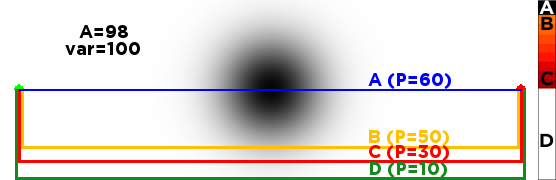
\includegraphics[width=\columnwidth]{graphix/SomePaths.png}
\caption{Gaussian paths with varying $P$, in relation to the Heat Map - As $P$ decreases from (A) to (D), the path gets further and further away. The direct path (A) is shown in black on the heatmap. Paths B and C with their positive finite $\yhat$ are shown in the heat map in color, with redder colors indicating longer paths. Path D reaches the edge of the simulation area, and as a result is the longest possible optimal path. It is shown in white on the heat map.}
\label{fig:somepaths}
\end{figure}

For the Gaussian non-lethal obstacle, the results of the simulation are a bit more complex. Let us start in Figure \ref{fig:somepaths} by changing the path constant as we did in Figure \ref{fig:gaussian} (although the scale is slightly different this time). Instead of showing all the paths, we can also represent this data as a heat map. The strip of a heat map in Figure \ref{fig:somepaths} shows varying values of $\yhat$ for a range of $P$ values. The discontinuity discussed in Figure \ref{fig:gaussian} is represented in the heat map by the quality of going from orange at path B straight to black for path A, skipping all the bluer values, i.e. the smaller $\yhat$ values. 

As is evident from Equation \ref{eq:PA}, $P$ and $V$ are inversely related. As long as the ration from $P$:$A$ remains constant, the value of $\yhat$ also remains constant (plots not shown). This means we can explore the entire parameter space as a two dimensional heat map relating that ratio to $\sigma$, as you can see in Figure \ref{fig:heatmap}. 

The first thing to note is the relationship between $\sigma$ and $\yhat$ for a given $P/A$. For any given finite positive value of $\yhat$ we can decrease the variance to get a smaller $\yhat$. This can be seen by picking any colored point in the heat map and moving to a smaller variance (down) and get a lower $\yhat$. However, the extent to which decreasing the variance will decrease $\yhat$ depends on the other variables. 

Increasing the variance (moving up), however, can result in multiple behaviors. As expected, increasing the variance will increase $\yhat$. Sometimes $\yhat$ will meet the edge of the grid, resulting in the white area. However, for the right portion of the heatmap, increasing the variance can actually \emph{decrease} the closest distance, all the way to $\yhat=0$. This corresponds with the fact the breakdown of our assumptions. For sufficiently large variances, our previous assumption that $n>>\sigma$ breaks down. For increasingly values of $\sigma$, $\yhat$ will eventually always be $0$. This makes sense because at that point the path is in the middle of the distribution, and the easiest path is merely to take the direct path. 

\begin{figure}
\centering
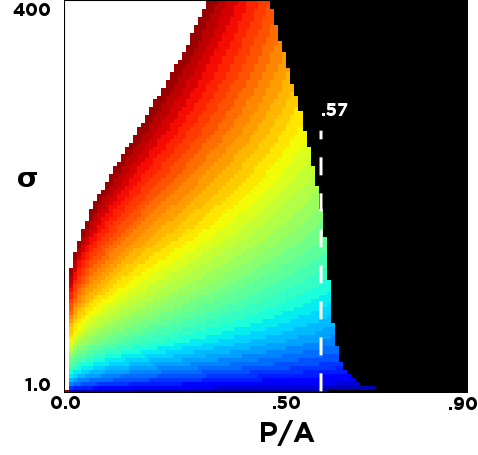
\includegraphics[width=.86\columnwidth]{graphix/heatmap.png}
\caption{Value of $\yhat$ for $P$/$A \times \sigma$}
\label{fig:heatmap}
\end{figure}

Turning our attention to $P/A$, our prediction was that $P/A > .57$ did not result in a solution to Equation \ref{eq:PA}, and ergo, $\yhat=0$. This is validated by the fact that most of the region to the right of the $P/A = .57$ line is black, representing $\yhat=0$. We have already seen how the assumptions of our solution break down as variance increases, explaining the black areas to the left of the $.57$ line. The reason for the area to the right of the line remains an open area of investigation. 

%Full heatmaps for different combinations of parameters are shown in Figure \ref{fig:colormaps}. For instance, according to equation (10), if $P/A$ is too high, there will be no solution and the optimal path will be at $\yhat=0$. We can see this in all four graphs of Figure \ref{fig:colormaps}, in that the black areas representing $\yhat=0$ appear for the large values of P and small values of A. We can also see in Figure \ref{fig:gap} that P and A have a linear relationship, which means that as long as the ratio of $P$:$A$ remains constant, the value of $\yhat$ will remain constant as well (given a particular variance). 

Lastly, it is worth noting that the $P$:$A$ ratio is vital to tuning the parameters. If the ratio is too high, there will be very few values for $\sigma$ that result in a usable $\yhat$. 

%relationship between amplitude and path constant is a key contributor to the ease of tuning parameters. Consider Figure \ref{fig:gav} where $P=10$ and Figure \ref{fig:gav2} where $P=25$. When $P$ is relatively low, there are many valid parameter combinations to get positive $\yhat$. However, with a higher $P$, there are significantly fewer options. In some cases, it does not matter what variance you dial in, $\yhat$ will not change from being 0. 

%\newcommand{\szsz}{.42}
%\begin{figure}[t]
%\centering
%\subfloat[Amplitude vs. Path Constant]{
%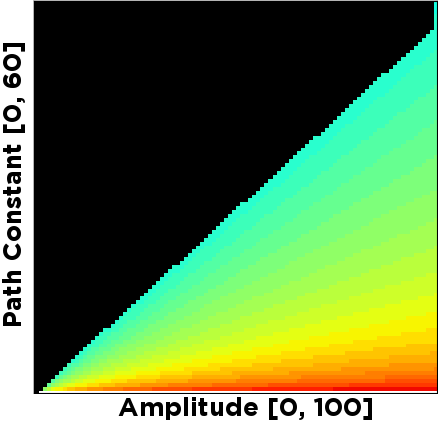
\includegraphics[width=\szsz\columnwidth]{graphix/gap.png}
%\label{fig:gap}}
%\qquad
%\subfloat[Variance vs. Path Constant]{
%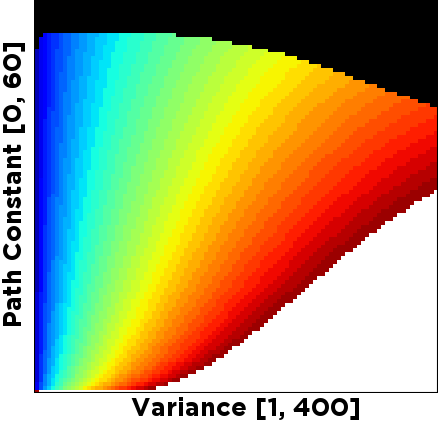
\includegraphics[width=\szsz\columnwidth]{graphix/gvp.png}
%\label{fig:gvp}}\\
%\subfloat[Amplitude vs. Variance \newline($P=10$)]{
%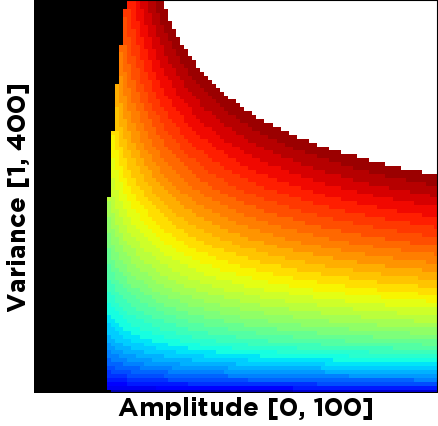
\includegraphics[width=\szsz\columnwidth]{graphix/gav.png}
%\label{fig:gav}}
%\qquad
%\subfloat[Amplitude vs. Variance \newline($P=25$)]{
%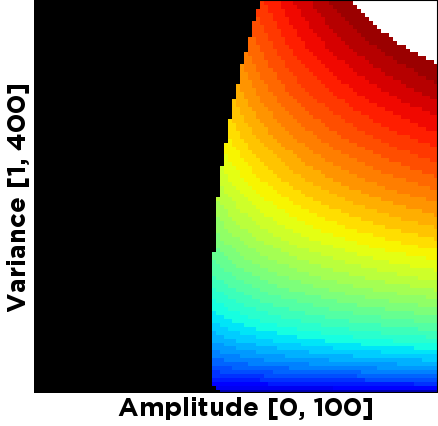
\includegraphics[width=\szsz\columnwidth]{graphix/gav2.png}
%\label{fig:gav2}}
%\caption{Heat Maps of $\yhat$ for different parameters for a Gaussian obstacle- The black areas mark where the path goes straight through the obstacle ($\yhat=0$), i.e. where the path constant is too high or the amplitude is too low. The white areas mark where the optimal path is as far away from the obstacle ($\yhat=\infty$), i.e. where the path traces the outer boundaries of the grid. Everything else is where $\yhat$ has a positive finite value, color coded with red paths being the longest and blue paths being the shortest.}
%\label{fig:colormaps}
%\end{figure}

